%!TEX root=../GaugeCNNTheory.tex


\section{Euclidean coordinate independent CNNs}
\label{sec:instantiations_euclidean}

This section considers equivariant convolutions on Euclidean (affine) spaces $M = \Euc_d$, which are undoubtedly of greatest practical relevance.
Convolutional network on Euclidean spaces are applied for analyzing planar and volumetric images, audio signals, videos, physical events in (pseudo-Euclidean) Minkowski spacetime or planar environments in reinforcement learning.
The prototypical convolutional model architecture -- both on Euclidean spaces and in general -- is the conventional CNN on~$\Euc_d$ by \citet{LeCun1990CNNs}.
Its success is to a large extent grounded in its translation equivariance, which allows it to generalize learned inference between different spatial locations.
Motivated by this observation, a lot of effort has been made to generalize the equivariance properties of CNNs to larger \emph{global} symmetry groups of~$\Euc_d$, for instance to the Euclidean isometries in Fig.~\ref{fig:isometries_plane} or more general affine transformations.


Interestingly, most of the \emph{globally} equivariant models in the literature achieve their equivariance by applying some kind of $G$-steerable kernels.
This implies that these models are actually equivariant under \emph{local} gauge transformations as well, despite not explicitly being designed for it.
The reason for this unintentional gauge equivariance is that the global equivariance of the models is usually designed for each layer individually, and therefore applies to the local receptive field of every neuron independently.
Here we explain globally equivariant Euclidean CNNs, listed in rows~(1-26) of Table~\ref{tab:network_instantiations}, from the more general viewpoint of local gauge symmetries and discuss how their global equivariance is induced from their local gauge equivariance.
Theorem~\ref{thm:isom_equiv_GM_conv} asserts thereby that a $\GM$-convolution on $M = \Euc_d$ is $\IsomGM$-equivariant.
However, for the specific case of Euclidean spaces, one can make a stronger statement than mere isometry equivariance:
the convolution with a $G$-steerable kernel on $\Euc_d$ implies the global equivariance of the model under the action of the affine group $\Aff(G) := \Trans_d \rtimes G$, as proven in Theorem~\ref{thm:affine_equivariance_Euclidean_GM_conv} below.
The underlying reason for this result is that the geodesics and Levi-Civita transporters are on Euclidean spaces not only preserved by isometries, but are more generally preserved by any affine transformation.

\begin{figure}
    \centering
    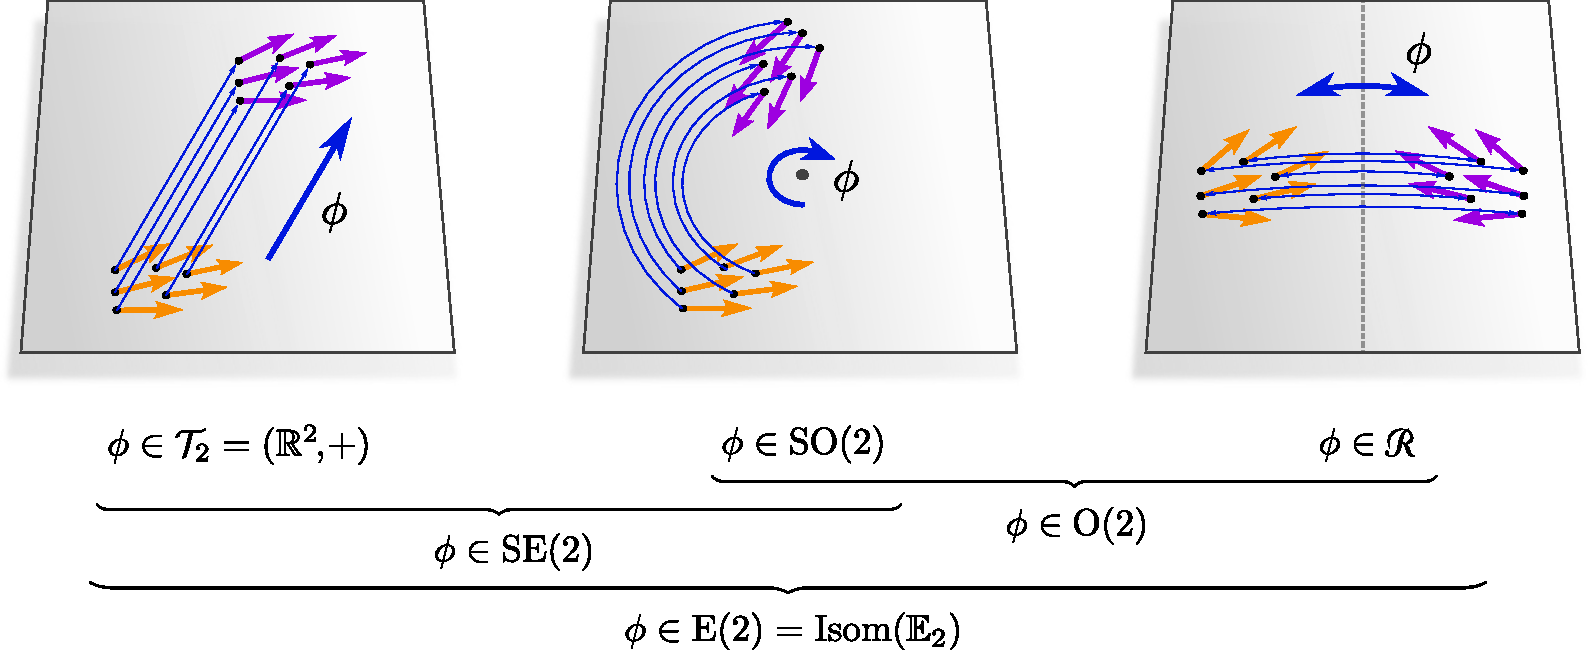
\includegraphics[width=1.\textwidth]{figures/isometry_plane.pdf}
    \vspace*{.1ex}
    \caption{\small
        Visualization of the full isometry group $\Isom(\Euc_d) = \E{d}$ of Euclidean spaces~$\Euc_d$ for $d=2$.
        It contains subgroups of translations $\Trans_d \mkern-1mu=\! (\R^d,\mkern-2mu+)$, rotations $\SO{d}$ and reflections $\Flip$.
        Rotations and reflections form the orthogonal group ${\O{d} \!=\! \SO{d} \!\rtimes\! \Flip}$ while translations and rotations form the special Euclidean group $\SE{d} = \Trans_d \rtimes \SO{d}$.
     }
    \label{fig:isometries_plane}
\end{figure}

Convolutions on Euclidean spaces are classically formulated \emph{in coordinates} $\R^d$ of $\Euc_d$.
The advantage of formulating convolutions this way is that $\R^d$ comes with all mathematical structure that is required for the definitions.
However, $\R^d$ is equipped with an excess of structure, for instance a vector space structure (and thus an origin) or its canonical $\{e\}$-structure.
By designing the convolutions to be equivariant, the inference is then (partly) made independent from this structure:
for example, the translation equivariance of convolutions equalizes the particular choice of origin while $\E{d}$ (isometry) equivariance equalizes the particular direction and orientation of the $\{e\}$-structure.
To clarify which mathematical structure is actually being assumed and required, we develop an alternative viewpoint:
we start out with the pure affine and metric structure of the Euclidean space~$\Euc_d$.
If~a $\GM$-convolution on $\Euc_d$ assumes more geometric structure, this structure will subsequently be added by specifying an atlases of (affine) charts $x^A: \Euc_d \to \R^d$, which induce gauges and $G$-structures.

\pagebreak

\etocsettocdepth{3}
\etocsettocstyle{}{} % from now on only local tocs
\localtableofcontents


To give an overview and a simple introduction, we review the classical formulation of $G$-steerable (affine equivariant) convolutions in coordinates $\R^d$ in Section~\ref{sec:steerable_cnns_in_coords}.
The following Sections~\ref{sec:euclidean_geometry} and~\ref{sec:euclidean_affine_equiv} define affine equivariant convolutions on Euclidean spaces in a coordinate free and coordinate independent setting.
Specifically, Section~\ref{sec:euclidean_geometry} discusses the affine geometry of Euclidean spaces.
Atlases of charts with transition functions in an affine group $\Aff(G)$ (Fig.~\ref{fig:affine_charts}) induce hereby the considered $\Aff(G)$-invariant $G$-structures (Fig.~\ref{fig:G_structures_R2_main}).
Section~\ref{sec:euclidean_affine_equiv} considers $\GM$-convolutions on these $G$-structures and proves their global $\Aff(G)$-equivariance.
The specific instantiations of such models found in the literature, i.e. rows~(1-26) of Table~\ref{tab:network_instantiations}, are discussed in Section~\ref{sec:euclidean_literature}.

The reader may choose to jump over the technical definitions in Sections~\ref{sec:euclidean_geometry} and~\ref{sec:euclidean_affine_equiv}, which are not strictly necessary to understand the models in Section~\ref{sec:euclidean_literature}.
